On considère à présent le cas d'un fluide réel pour lequel $\epsilon>0$. On traite le problème dans l'approximation dite de champ moyen. Pour ce faire on réécrit l'hamiltonien ci-dessus en utilisant la décomposition suivante
$$
n_i n_j = (n_i -n)(n_j -n)+ n(n_i+n_j)-n^2
$$
où $n=\frac{N}{M}$ est le taux moyen d'occupation d'un site, qui est {\it indépendant} du site considéré.

\question
L'approximation de champ moyen consiste à négliger le terme de fluctuation
$$
\sum_{\langle i,j\rangle} (n_i -n)(n_j -n)
$$
Montrer que l'hamiltonien du fluide s'écrit alors comme une somme d'hamiltoniens indépendants~:
$$
H \simeq \sum_{i=1}^{M}\bigg(-6\epsilon n n_i+ 3\epsilon n^2 \bigg)
$$
Donner une interprétation du \og champ moyen\fg.

\question
Calculer la grande fonction de partition $\Xi(\mu,T,n)$ et le grand potentiel $J(\mu,T,n)$ pour $n$ {\it fixé}.

\question
Exprimer le taux moyen d'occupation d'un site sous la forme d'une équation auto-cohérente : $n=f(n)$.

\question
Montrer que l'équation d'état du fluide est donnée par~:
$$
P=-\frac{k_BT}{v_0} \ln(1-n) -\frac{3\epsilon} {v_0}n^2 =-\frac{k_BT}{v_0} \ln(1-v_0\rho) -3\epsilon v_0 \rho^2
$$
où $\rho=\frac{N}{V}$ est la densité du fluide. 

\question
Calculer le coefficient du Viriel $B_2(T)$ à partir de l'équation d'état. Son expression était-elle attendue ? Montrer que l'on retrouve le même comportement pour $B_2(T)$ que dans l'équation d'état de van der Waals.

\question
L'isotherme critique du CO$_2$ est représentée sur la figure ci-dessous. Commenter la validité de l'approximation du gaz parfait et celle du modèle de gaz sur réseau en champ moyen étudié dans cet exercice.


\begin{figure}[h!]
  \centering
  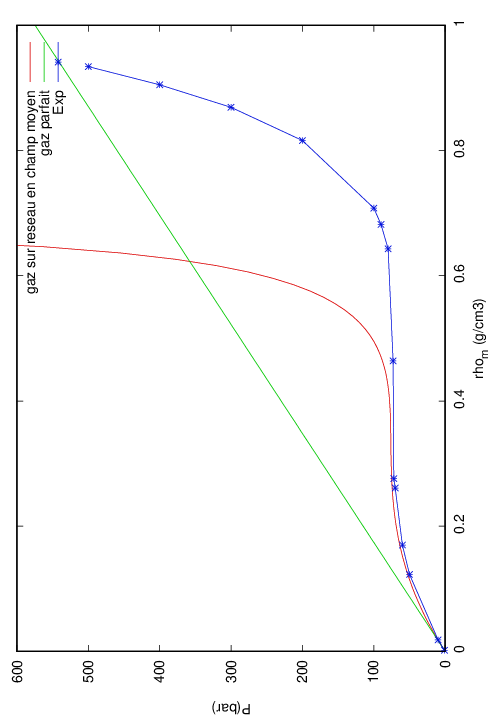
\includegraphics[scale=.7,angle=-90]{../Fig/CO2}
  \caption{Isotherme critique $P(\rho_m)$ du CO$_2$ à $T=T_c=304$ K
    pour le gaz parfait (ligne droite) et pour le gaz sur réseau en
    champ moyen donnée par l'équation de $H_{gr}$ (en trait
    plein), avec des valeurs ajustées de $v_0$ et de $\epsilon/k_B$. Les données expérimentales
    sont représentées par des croix. La pression est exprimée en bar
    et la masse volumique, $\rho_m$, en g.cm$^{-3}$. La masse
    volumique critique est $\rho_{m_{c}}=0,46$ g.cm$^{-3}$.}
\end{figure}


\question
Montrer que si $T$ est inférieure à une température critique $T_c$, le système peut devenir instable, c'est-à-dire que sa compressibilité isotherme
$$
\kappa =-\frac{1}{V} \frac{\partial V}{\partial P}\bigg|_T= \frac{1}{\rho} \frac{\partial \rho}{\partial P}\bigg|_T
$$
est négative pour certaines valeurs de la densité.  Déterminer les coordonnées $T_c$, $P_c$ et $\rho_c$ du point critique. Le facteur de compressibilité critique défini par $\displaystyle Z_c=\frac{P_c}{k_BT_c\rho_c}$ dépend-il du fluide considéré ? Comparer sa valeur à celle mesurée pour le CO$_2$ : $Z_c\simeq 0,27$.

